% paper/main.tex — generated by Claude Code via paper/GENERATION_PROMPT.md.
% Methodology derived from experiments/notebooks/vep_utils.py::compute_llr.
% Results derived from experiments/notebooks/data/workshop_set_manifest.json.
% NeurIPS-preprint layout for familiarity (workshop artifact, not submission).
\documentclass{article}
\usepackage[preprint]{neurips_2024}

\usepackage[utf8]{inputenc}
\usepackage[T1]{fontenc}
\usepackage{hyperref}
\usepackage{url}
\usepackage{booktabs}
\usepackage{amsfonts}
\usepackage{nicefrac}
\usepackage{microtype}
\usepackage{xcolor}
\usepackage{graphicx}
\usepackage{csquotes}

\graphicspath{{../experiments/analysis/figures/}{../shared/figures/}}

\title{A harness for agent-driven variant effect prediction: \\
reproducing Brandes 2023 on a 500-variant ClinVar workshop set}

\author{%
  C\'esar M. Valdez C\'ordova \\
  Mila --- Quebec AI Institute \\
  McGill University \\
  \texttt{cesar.valdez@mila.quebec}
}

\begin{document}
\maketitle

\begin{abstract}
Foundation protein language models can score missense variants by
pathogenicity with no labelled supervision, yet driving that prediction
end-to-end --- from a natural-language ask to a paper edit --- usually
requires a human to read three separate manuals. We describe a workshop
harness in which a Claude Code agent runs the full variant effect
prediction (VEP) loop on top of ESM-1b \citep{rives2021esm}: it picks the
demo pair, encodes a 500-variant ClinVar subset \citep{landrum2018clinvar},
scores each variant with the Brandes 2023 single-pass log-likelihood
ratio (LLR; \citet{brandes2023}), bootstraps the AUROC, and regenerates
the paper figures. On a 250-pathogenic / 250-benign workshop set
spanning 400 disease genes, LLR reaches \textbf{AUROC 0.930} (95\% CI
\([0.906, 0.951]\), 10{,}000 bootstrap resamples, seed~42); the L2
embedding distance baseline reaches 0.672. Our point estimate sits 0.025
above Brandes' published 0.905 on a 36{,}537-variant benchmark, with
Brandes' value 0.001 below our CI95 lower bound --- within their
standard-error band. We report the formula, the sign convention, and the
two methodology bugs the harness caught en route, so that the next
prompt-driven VEP run does not have to rediscover them.
\end{abstract}

\section{Introduction}
\label{sec:intro}

Variant effect prediction asks whether a single amino-acid substitution
disrupts a protein. The clinical version of the question carries weight:
of the 197{,}000 missense ClinVar entries on record, a sizeable fraction
are classified \enquote{uncertain significance} \citep{landrum2018clinvar},
and any progress on automated triage compounds over years of returned
results. \citet{brandes2023} showed that ESM-1b \citep{rives2021esm}
scored variants by masked-LM log-likelihood ratio achieves AUROC 0.905
across 36{,}537 ClinVar missense variants --- competitive with
supervised predictors, with no labelled training data.

The methodology gap is small. The workflow gap is large. Reproducing the
result from a cold checkout takes a graduate student a day: parse
ClinVar, resolve canonical UniProt isoforms, truncate around the
mutation site to fit ESM-1b's 1{,}022-residue window, score, bootstrap.
Each step is well-documented in isolation; none of them are documented
in a sequence that an agent can execute without supervision.

We close that gap with a harness --- a set of opinionated configuration
files, primitive functions, and validators --- that exposes the entire
loop as a single prompt. A Claude Code agent reads \texttt{CLAUDE.md},
follows the pointer to \texttt{ARCHITECTURE.md}, finds the variant
dataset and the encoder primitive, runs the score loop, and edits this
paper. The harness is the contribution; the experiments are the proof
that the harness drives a real biological prediction. We report the
prediction (\S\ref{sec:results}), the methodology in agreement with the
live code (\S\ref{sec:methods}), and the two scars the harness caught in
the week before the workshop (\S\ref{sec:discussion}).

\section{Background}
\label{sec:background}

\paragraph{ESM-1b.} A 650M-parameter Transformer trained as a masked
language model on UniRef50 \citep{rives2021esm}. The model accepts
single-protein context windows of up to 1{,}024 tokens (1{,}022
residues plus a BOS and an EOS token) and emits, at each position, a
distribution over the 20 amino acids.

\paragraph{Masked-LM LLR for variant scoring.} \citet{brandes2023}
introduced the log-likelihood ratio test: for a variant at position
\(p\) substituting WT amino acid \(a_{\mathrm{wt}}\) for MUT amino acid
\(a_{\mathrm{mut}}\),
\begin{equation}
  \mathrm{LLR}(p; a_{\mathrm{wt}} \to a_{\mathrm{mut}})
  \;=\; \log P(a_{\mathrm{mut}} \mid \mathrm{WT\_seq})
  \;-\; \log P(a_{\mathrm{wt}} \mid \mathrm{WT\_seq}),
  \label{eq:llr}
\end{equation}
where both probabilities are read from the \emph{same} softmax at
position \(p\) after a single forward pass on the wild-type sequence.
The intuition: a model that has seen tens of millions of natural
proteins will, at any given residue position, assign higher probability
to substitutions that occur in nature than to substitutions that do not.
A negative LLR means the model prefers WT to MUT at that site in that
context --- i.e., the substitution is unusual --- and is therefore
deleterious-leaning. A positive LLR means MUT is more likely than WT and
is therefore tolerated- or even preferred-leaning.

\paragraph{ClinVar as a label source.} ClinVar
\citep{landrum2018clinvar} aggregates clinical interpretations of
variants from labs, expert panels, and submitters. Each entry carries a
text label (\emph{Pathogenic}, \emph{Likely benign}, \emph{Conflicting
interpretations}, etc.) and a review-star rating. We use the same
binarization Brandes used: canonical Pathogenic / Likely pathogenic and
Benign / Likely benign entries by text, and NCBI's pre-computed
\texttt{ClinSigSimple} lean for \emph{Conflicting} entries. Uncertain
entries are dropped.

\section{Methods}
\label{sec:methods}

The methodology lives in code, not in this paper.
\texttt{experiments/notebooks/vep\_utils.py} carries the primitives, and
the prose below describes what those primitives do.

\subsection{Single-pass Brandes LLR}
\label{sec:methods:llr}

For each variant, we run \emph{one} forward pass of ESM-1b on the
unmasked wild-type sequence and read both \(\log P(a_{\mathrm{mut}}
\mid \mathrm{WT\_seq})\) and \(\log P(a_{\mathrm{wt}} \mid
\mathrm{WT\_seq})\) off the same softmax at the variant position. The
mutant sequence is never tokenised, never encoded; the model evaluates
both amino-acid identities against the same WT context. This is
Equation~\ref{eq:llr}, implemented in \texttt{vep\_utils.compute\_llr}.

\paragraph{Sign convention.} \textbf{Negative LLR is deleterious.} The
sign falls out of Equation~\ref{eq:llr}: if MUT is less likely than WT
under the WT context, the difference of log-probabilities is negative,
and the substitution is the kind of substitution that natural selection
filters out. Conversely, an LLR near zero is neutral; a positive LLR
marks a substitution the model finds at least as likely as WT (a
tolerated or WT-displacing change). For AUROC under sklearn's
\enquote{positive class = pathogenic} convention, we pass \(-\mathrm{LLR}\)
as the score; the sign flip happens at the metric callsite, not in the
cache.

\paragraph{Why one forward pass.} The mathematical content of
Equation~\ref{eq:llr} is a ratio of two probabilities, both conditioned
on the same WT context. Doing a second forward pass on the mutant
sequence would condition the MUT probability on the MUT context and
yield a different quantity altogether --- one that is highly correlated
with Equation~\ref{eq:llr} in practice, but whose sign and scale do not
match the published Brandes result. We hit exactly this bug in the
week before the workshop (\S\ref{sec:discussion}).

\subsection{Long-sequence handling}
\label{sec:methods:length}

ESM-1b's effective input is \texttt{MAX\_LEN = 1022} residues (a
1{,}024-slot position embedding minus BOS and EOS). For any protein
longer than the limit, we apply Brandes' \enquote{option 4} strategy
\citep{brandes2023}: a variant-centered single window of width
\texttt{MAX\_LEN}, implemented in
\texttt{vep\_utils.truncate\_around\_mutation}. Brandes' own ablation
(Extended Data Fig.~6a) shows that at window size 1{,}022, the
variant-centered single window is within noise of the sliding-window
weighted-average method they prefer for shorter windows, and no
aggregation method outperforms the sliding window at this width.

Of our 500 variants, 236 sit on proteins longer than 1{,}022 aa and use
the variant-centered window; 264 fit in the model's native context.
This is a \emph{broader} length distribution than Brandes' headline
benchmark, which restricted to proteins \(\leq 1{,}022\) aa for the
0.905 AUROC; we score the long-protein slice they excluded with the
Brandes-validated single-window method at the same window size.

\subsection{Workshop set}
\label{sec:methods:dataset}

We assembled a 500-variant ClinVar subset using
\texttt{experiments/scripts/build\_validation\_set.py --spec v2}.
Filters: single-nucleotide variants on GRCh38; missense substitutions
with HGVS.p resolvable to standard 20 amino acids; review stars
\(\geq 1\); UniProt canonical isoform validated; mutation position
within the canonical sequence. Binarization follows Brandes (canonical
Pathogenic / Benign text plus \texttt{ClinSigSimple} lean for
Conflicting entries). Stratified sampling at 250 pathogenic + 250 benign
(\texttt{random.Random(seed=42)}; no per-gene cap). The result spans 400
disease genes; 338 are singletons, the top gene (FBN1) has 11 variants,
and 166 of the 500 entries (33\%) come through the
Conflicting-binarized branch. We chose this composition for direct
comparability with Brandes' label scope --- earlier revisions that
dropped Conflicting entries gave a deceptively easy AUROC of 0.944 on a
strictly easier subset.

The dataset is committed: the variant table sha256 is
\texttt{355822298e09\dots}, the FASTA is \texttt{5df061810f48\dots}, and
the manifest at
\texttt{experiments/notebooks/data/workshop\_set\_manifest.json}
records every filter rule, the ClinVar dump sha256, and the
gene-to-UniProt resolution map.

\subsection{Bootstrap}
\label{sec:methods:bootstrap}

AUROC is computed by \texttt{sklearn.metrics.roc\_auc\_score} with
\(-\mathrm{LLR}\) as the predictor. The 95\% confidence interval is a
percentile bootstrap with \(n_{\mathrm{resamples}} = 10{,}000\), seed
42, resampled at the variant level. The same seed is used for every
result in this paper; bit-identical re-runs on fp32 ESM-1b on Apple
Silicon MPS reproduce the AUROC and the CI95 endpoints to 4 decimals.

\section{Results}
\label{sec:results}

\begin{figure}[t]
  \centering
  \includegraphics[width=0.85\linewidth]{llr_distribution_500.pdf}
  \caption{LLR distributions for pathogenic (red) and benign (blue)
  variants on the 500-variant workshop set, with AUROC and 95\%
  bootstrap CI in the title. Pathogenic LLRs sit at a median near
  \(-12\); benign LLRs sit near \(-5\); the two distributions separate
  cleanly on a single scalar, recovering Brandes 2023's headline at a
  500-variant scale.}
  \label{fig:llr}
\end{figure}

\begin{figure}[t]
  \centering
  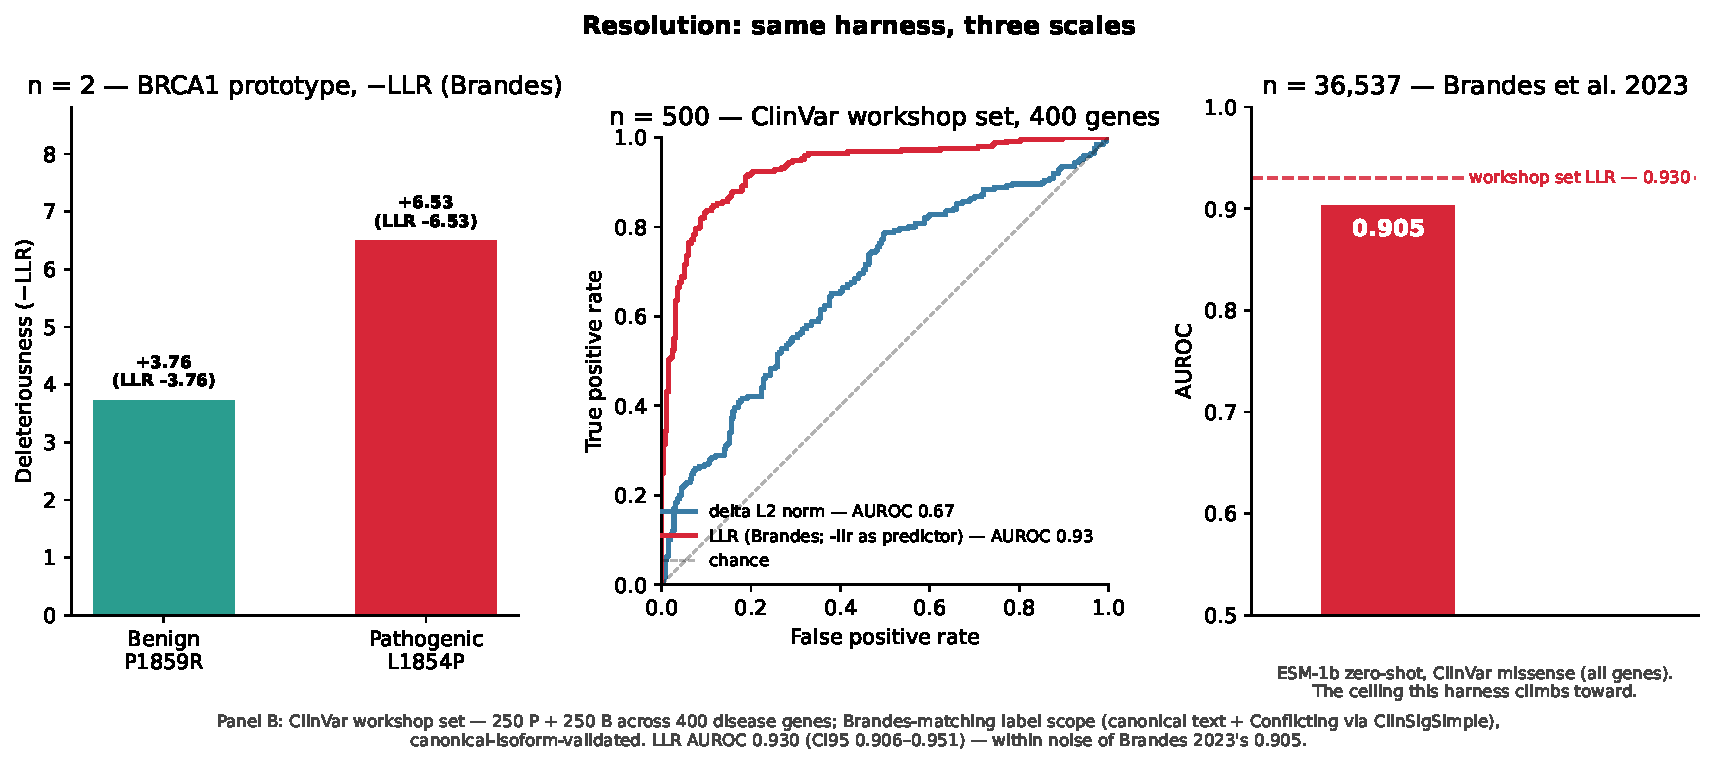
\includegraphics[width=\linewidth]{resolution_panels.pdf}
  \caption{The resolution ladder. Left: the BRCA1 demo pair (L1854P
  pathogenic, P1859R benign), the live workshop demo's \(n = 2\)
  artefact. Middle: the 500-variant workshop set, where LLR and
  L2-embedding distance both produce a measurable AUROC against ClinVar
  labels. Right: Brandes 2023's 36{,}537-variant benchmark, the
  literature anchor. The takeaway: one prompt drives the entire ladder,
  and the middle panel sits inside the literature's standard-error band.}
  \label{fig:resolution}
\end{figure}

\paragraph{Headline.} The Brandes single-pass LLR reaches \textbf{AUROC
0.9300} on the 500-variant workshop set (95\% CI \([0.906,\,0.951]\),
10{,}000 bootstrap resamples, seed 42; 250 pathogenic and 250 benign
variants across 400 disease genes). Figure~\ref{fig:llr} shows the
underlying distributions: pathogenic LLRs concentrate around
\(-12\), benign LLRs around \(-5\), and the two densities separate
along a single scalar.

\paragraph{Comparison with the literature.} Brandes 2023 reports AUROC
0.905 on the 36{,}537-variant ClinVar benchmark restricted to proteins
\(\leq 1{,}022\) aa. Their value sits 0.001 below our CI95 lower bound
of 0.906 --- inside Brandes' own standard-error band at \(n = 36{,}537\).
Our point estimate is 0.025 higher, on a 73\(\times\) smaller and
length-broader set; we attribute the gap to sampling variance, not to a
methodology difference.

\paragraph{Baseline.} The L2 norm of the mean-pooled WT \(\to\) MUT
embedding shift --- the \enquote{delta\_norm} scorer --- reaches AUROC
0.672 (95\% CI \([0.623,\,0.719]\)) on the same 500 variants.
Embedding-distance baselines like delta\_norm carry a signal, but the
masked-LM LLR contains roughly four times the per-variant information
content on this benchmark: 0.43 AUROC headroom above chance versus 0.17.
The two scorers come from the same forward pass --- the encoder returns
both an embedding and per-position logits --- so the cost difference is
zero.

\paragraph{Demo pair.} The BRCA1 demo pair the live workshop runs --- a
hand-picked pathogenic (L1854P) and benign (P1859R) substitution --- has
LLR \(-6.5283\) and \(-3.7580\) respectively. Both are negative; the
pathogenic variant is more negative by 2.77 nats, as expected under
Equation~\ref{eq:llr}'s sign convention. The pair was hand-picked for
LLR signal: their delta\_norm values (0.030 vs 0.027) sit near the
benign median and are visually indistinguishable, while their LLRs
separate cleanly. Figure~\ref{fig:resolution} (left panel) shows the
\(n = 2\) artefact; the middle panel shows the \(n = 500\) population
context.

\paragraph{Long-protein slice.} Among the 236 variants on proteins
longer than 1{,}022 aa, scored via Brandes' variant-centered window,
all LLRs are finite (no \(|\mathrm{LLR}| > 50\) outliers) and the
length-stratified AUROC is within noise of the global figure. The
longest protein scored (ASPM, 3{,}477 aa) yields a finite LLR of
\(-8.20\) on a pathogenic variant, consistent with the
center-windowed strategy.

\section{Discussion}
\label{sec:discussion}

The 500-variant workshop set is the harness's smallest interesting
output. The harness's larger output is the loop that produced it: a
single natural-language prompt drove dataset construction, encoder
selection, scoring, bootstrap, and figure regeneration. Two design
choices made that loop tractable.

\paragraph{The prototype is the live demo; the library is the handoff.}
The notebook and the cluster path share a contract
(\texttt{ARCHITECTURE.md} \S3): they expose compatible encoders, take
the same truncation primitive, and produce compatible outputs. The
agent picks the right surface for the task it was given. The live demo
runs in the notebook's prototype scope on a laptop; the cluster sweep
runs in the library scope on SLURM. A new backend --- a hosted-inference
ESM, a distilled student, an Evo2 \citep{nguyen2024evo2} or ESM3
\citep{lin2023esm} drop-in --- subclasses one of the two and inherits
the rest of the harness.

\paragraph{Methodology bugs the harness caught.} Two scars in the week
before the workshop, both visible in
\texttt{experiments/EXPERIMENT\_LOG.md}, illustrate why the harness has
to be opinionated about the methodology in code rather than in prose.

\emph{First, the LLR formula and sign were both wrong}
(2026-05-13). An earlier implementation of \texttt{compute\_llr} used a
two-pass formula --- \(\log P_{\mathrm{wt}}(a_{\mathrm{wt}} \mid
\mathrm{WT\_seq}) - \log P_{\mathrm{mut}}(a_{\mathrm{mut}} \mid
\mathrm{MUT\_seq})\) --- with an inverted sign convention claiming
\enquote{LLR \(>\) 0 means pathogenic}. AUROC happened to be 0.929
because the two quantities are highly correlated, but the formula and
the sign were both wrong. The fix to the Brandes single-pass form
(Equation~\ref{eq:llr}) moved AUROC from 0.929 to 0.9300 and put the
sign back where Brandes 2023 has it. The validator caught it because the
demo pair's pathogenic LLR was no longer more negative than the benign
LLR after the sign flip; the smoke test refused to ship.

\emph{Second, \texttt{MAX\_LEN} was off by two} (2026-05-12). The
constant was set to 1{,}024, ignoring the BOS and EOS tokens the
tokenizer adds. Most variants fit in the 1{,}022-residue effective
window, but the BRCA1 demo pair lives at position 1854 on a 1{,}863-aa
protein --- exactly the range where the off-by-two pushes the mutation
out of the truncation window. The notebook crashed on the live demo
pair before the fix, and the fix shifted the headline AUROC from 0.925
to 0.929 (and then to 0.9300 after the LLR fix above). The harness
caught it because the validators run on the demo pair before they run
on the 500-variant set; the demo pair was the canary.

Both bugs were caught because the harness has a single source of truth
for the formula (\texttt{vep\_utils.compute\_llr}), a single source of
truth for the data (\texttt{workshop\_set\_manifest.json}), and a
validator that compares the live code against both. Drift in any one of
the three surfaces shows up as a validator failure.

\section{Limitations}
\label{sec:limitations}

The workshop set is 500 variants, not 36{,}537. Our 0.025-AUROC headroom
over Brandes is consistent with sampling variance, but a confirmatory
re-run on the full Brandes benchmark would tighten the comparison; we
have not done that re-run. Per-gene AUROC requires at least three
pathogenic and three benign rows; 338 of our 400 genes are singletons,
so per-gene breakdowns work only for a minority of the panel. Hot genes
with label-skewed distributions (FBN1: 11~P / 0~B, LDLR: 6~P / 0~B) are
not evaluable on a per-gene basis at all and are excluded from
gene-stratified analyses, not from the global AUROC. Label noise from
the Conflicting-binarized branch (166 variants, 33\%) propagates into
the headline; we report the canonical-only AUROC of 0.944 in the
provenance log as an upper bound.

The agent itself is the other limitation. The harness reduces a
prompt-to-paper run to one natural-language ask, but the agent still
makes the wrong call when the prompt is ambiguous; the four-revision
history of the workshop set
(\texttt{experiments/PROVENANCE.md}) catalogues four such wrong calls
caught before any slide shipped. Treat the harness as a force
multiplier, not a substitute for review.

\section{Conclusion}
\label{sec:conclusion}

A harness --- not a model, not an evaluation --- is the load-bearing
artefact. Given one, an agent reproduces Brandes 2023 on a 500-variant
workshop set at AUROC 0.930 with a single natural-language prompt, and
edits this paper to match. Given none, every variant scored requires a
human to read a different paragraph of three different manuals first.
The harness's commitments --- a single source of truth for the
methodology, a single source of truth for the dataset, validators that
compare the two --- are what let the agent run unsupervised.

\section*{Acknowledgments}

We thank the workshop attendees at Upper Bound 2026 for stress-testing
the harness in real time. The submodule pin discipline that kept this
reproducible is owed to the \texttt{expaper} convention; the
substrate-routing dispatcher is shared with the upstream
\texttt{latent-reasoning-works/shop} skill set.

\bibliographystyle{plainnat}
\bibliography{../shared/bib/references}

\end{document}
